\documentclass{article}

\usepackage[utf8]{inputenc}
\usepackage[german]{babel}
\usepackage{amsmath}
\usepackage{mathtools}
\usepackage{listings}
\usepackage{color}

\lstset{
  language=C,                     % choose the language of the code
  numbers=left,                   % where to put the line-numbers
  stepnumber=1,                   % the step between two line-numbers.        
  numbersep=5pt,                  % how far the line-numbers are from the code
  backgroundcolor=\color{white},  % choose the background color. You must add \usepackage{color}
  showspaces=false,               % show spaces adding particular underscores
  showstringspaces=false,         % underline spaces within strings
  showtabs=false,                 % show tabs within strings adding particular underscores
  tabsize=2,                      % sets default tabsize to 2 spaces
  captionpos=b,                   % sets the caption-position to bottom
  breaklines=true,                % sets automatic line breaking
  breakatwhitespace=true,         % sets if automatic breaks should only happen at whitespace
  title=\lstname,                 % show the filename of files included with \lstinputlisting;
}

\begin{document}

\tableofcontents

\section{Betriebssystem}

\subsection{Definition}

\begin{itemize}
    \item \textbf{Systemsicht} \\
        Alle Programme zur \textbf{Steuerung und Überwachung} von:
        \begin{itemize}
            \item Ausführung v. Benutzerprogrammen
            \item Verteilung der Betriebsmittel
            \item Aufrechterhaltung der Betriebsart
        \end{itemize}
    \item \textbf{Anwendersicht} \\
        \textbf{Virtuelle Maschine}, vereinfachte Ansicht des Computers
\end{itemize}

\subsection{Aufgaben}

\begin{itemize}
    \item \textbf{Hardwareabstraktion}
    \begin{itemize}
        \item einheitliche Sicht auf Geräteklassen
        \item Bibliotheken und Treiber
    \end{itemize}

    \item \textbf{Resourcenverwaltung}
    \begin{itemize}
        \item CPU-Rechenzeit
        \item Speicher
        \item Gerätezugriffe
    \end{itemize}

    \item \textbf{Sicherheitsfeatures}
    \begin{itemize}
        \item Benutzer und Gruppen \textbf{Multi-User}
        \item Parallelbetrieb \textbf{Multitasking}
        \item Schutz for direkten Hardwarezugriffen
    \end{itemize}
\end{itemize}

\subsection{Arten}
\begin{itemize}
    \item \textbf{Mainframe}
        schnelles I/O, viele Prozesse, Transaktionen
    \item \textbf{Server}
        viele Anwender, Netzanbindung    
    \item \textbf{Multiprozessor}
    \item \textbf{Echtzeit}
\end{itemize}

\section{Prozesse}

\subsection{Bestandteile}
\begin{itemize}
    \item eigener Adressraum
    \item Programmcode
    \item Programmdaten
    \item Programm-Counter
    \item Stacks und Stackpointer
    \item Hardwareregister-Inhalte \textit{(Prozess-Kontext)}
    \item Heap-Speicher
    \item Verwaltungsdaten
    \begin{itemize}
        \item Identifier und VaterID
        \item Resourcenliste
        \item Scheduling Parameter
    \end{itemize}
\end{itemize}

\begin{figure}[ht!]
    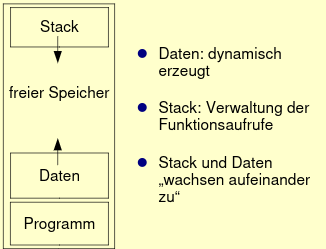
\includegraphics[scale=.75]{pics/processes}
    \caption{Process Control Block PCB}
\end{figure}

\subsection{Hierarchie und Signale}
Jeder Prozess hat \textbf{Vaterprozess} \textit{(Prozesse erzeugen einander)}.

\subsubsection{Fork}
\begin{lstlisting}
    int pid = fork();
    if(pid == 0){
        printf("Ich bin das Kind mit pid=%d\n", getpid());
    }else if(pid > 0){
        printf("Ich bin der Vater, mein Kind hat die pid=%d\n", pid);
    }else{
        printf("Error: fork() war nicht erfolgreich");
    }
\end{lstlisting}

\subsubsection{Signale}
\begin{itemize}
    \item (17) STOP \textit{(Strg-Z oder bg)}
    \item (19) CONT \textit{(fg)}
    \item (15) SIGTERM \textit{(beenden)}
    \item (9) KILL \textit{(abschließen)}
\end{itemize}

\subsection{Prozesserzeugung}
\begin{enumerate}
    \item fork $\rightarrow$ clone $\rightarrow$ do\_fork $\rightarrow$ copy\_process
    \item neue thread\_info in task\_struct
    \item Kind-Status auf TASK\_UNINTERRUPTABLE
    \item copy\_flags
    \item get\_pid: neue PID für Kind
    \item je nach clone-Parametern: kopieren/gemeinsam nutzen
    \item Scheduler
\end{enumerate}

\end{document}
